\chapter{Constrained keyframe Localization and mapping (CKLAM)}
\label{sec:CKLAM}
\section{Bundle Adjustment Overview}
In this chapter we shall take a look at the core concepts and equations of CKLAM proposed in \cite{CKLAM}, in order to understand the design and the associated advantages/ disadvantages. In order to do that we shall look a the the necessary parts of Bundle Adjustment. 
A bundle adjustment problem of a visual inertial map (VIMAP) is nothing but a complete optimization problem given all exteroceptive and interoceptive measurements, essentially producing a maximum a posteriory (MAP) estimation of the state variable. For readability let us consider that our map consists of only five camera poses and only five features. The measurements and visibility of landmarks is shown in figure \ref{fig:CKLAM_BLOCK}. 

\begin{figure}[ht]
	\centering
		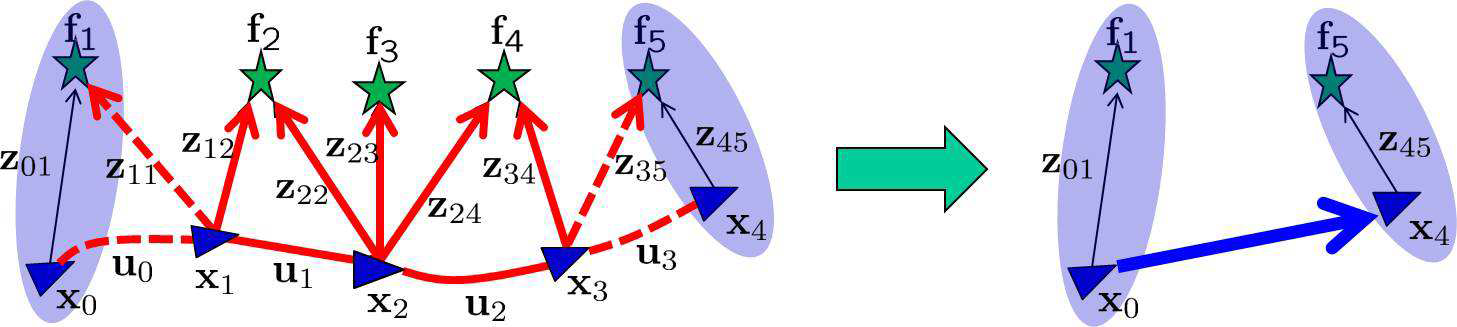
\includegraphics[width=1.00\textwidth]{images/cklam_block.png}
		\caption{An example of the exploration epoch before (left) and after (right) the approximation employed in CKLAM. $x_0$, $x4$ are the key-frames to be retained, and $x_1$, $x_2$, and $x_3$ are the non-key-frames to be marginalized. Similarly, $f_1$, $f_5$ are key landmarks (observed from the key-frames) to be retained, while $f_2$, $f_3$, and $f_4$ are non-key landmarks (observed exclusively from the non-key-frames) to be marginalized. In the left figure, the arrows denote the measurements between different states. In the right figure, the blue arrow represents the pose constraint generated between the key-frames using C-KLAM. \cite{CKLAM} }
	\label{fig:CKLAM_BLOCK}
\end{figure}

In figure \ref{fig:CKLAM_BLOCK} $z_{ij}$ denote the set of exteroceptive measurements from pose $x_i$ to landmark $f_j$ also let $u_i$ denote the proprioceptive measurement from $x_i$. The objective in this setting would be to perform an $argmin$ operation on the cost function $C$ given by Eq.( \ref{BA_FULL_COST}). 

\begin{equation}
  C = f(x_{0:4}, f_{1:5}, u_{0:3}, z_{0:4, 1:5}) = f_1(x_0, x_4, z_{01}, z_{45}, f_1, f_5) + f_2(x_{0:4}, f_{1:5}, z_{1:3, 1:5})
  \label{BA_FULL_COST}
\end{equation}

In a more concrete way this cost function can also be written as in Eq.(\ref{BA_FULL_COST_REWRITTEN}). Clearly every measurement here contributes one residual term and we perform an $argmin$ operation on the final squared residual. It can be seen that the number of such residual term for such a problem is addition of number of camera poses and number of landmarks observed form each of these poses, which are often very high in real life maps. A typical small map of duration of about a minute can have more than $1000$ robot pose and $12000$ IMU measurements and more than $50000$ landmarks. Hence the $argmin$ operation on a map of this size is quite computation intensive. In order to perform bundle adjustment in reasonable time traditionally selected robot poses and associated observations are discarded. For instance in figure \ref{fig:CKLAM_BLOCK} we decided to discard poses $x_1$ through $x_3$ as well as $f_2$ through $f_4$. This leads to dramatic reduction in computational complexity by crucial information from non-key-frames is lost. CKLAM attempts to preserve this information by projecting them into the retained frames. The newly computed information is represented by the blue arrow from $x_0$ to $x_4$ in the right half of figure \ref{fig:CKLAM_BLOCK}

\section{CKLAM Formulation}
As stated earlier the objctive of CKLAM is to retain information from the poses that we have selected to eliminate such that we can achieve computational complexity reduction while retaining high quality of optimization result. If we look closely it is not hard to notice that the two terms of Eq.(\ref{BA_FULL_COST}) correspond to the two different part of the optimization problem in hand, viz. the first part i.e. $f_1$ comes from the terms that we intend to retain after CKLAM process while the the second part $f_2$ is the contribution of the poses and landmarks that we intend to eliminate from the optimization. In order to perform this elimination process let us define the second term of second part of the Eq.(\ref{BA_FULL_COST}) to be $C_2$, formally given in Eq. (\ref{FULL_C2_COST}). 

Since $C_2$ depends not only on the key-frame poses viz. ($x_{0,4}$) but also upon poses ($x_{1:3}$) that we would like to eliminate/marginalize, we have to find an approximation $C_2^{'}$ such that $C_2^{'}$ would depend only on the key-frame poses and landmarks that we intend to retain, i.e. $x_0$, $x_4$, $f_1$ and $f_5$. 

\begin{equation}
C_2 = f_2(x_{1:4}, f_{1:5}, z_{1:3, 1:5})
\label{FULL_C2_COST}
\end{equation}

In order to perform this elimination/marginalization step let us approximate $C_2$ with a quadratic function as shown in in Eq.(\ref{C2_APPROX}). This can easily be achieved by tailor expanding the function $f_2$.

\begin{equation}
\begin{split}
C_2 \approx \alpha + g^T\begin{bmatrix} x_{0:4} - \hat x_{0:4} \\ 
                                  f_{1:5} - \hat f_{1:5}\\
									\end{bmatrix} 
									+ \frac{1}{2} \begin{bmatrix} x_{0:4} - \hat x_{0:4} \\ 
                                        f_{1:5} - \hat f_{1:5}\\
									              \end{bmatrix}^T H 
												\begin{bmatrix} x_{0:4} - \hat x_{0:4} \\ 
                                        f_{1:5} - \hat f_{1:5}\\
									      \end{bmatrix} = \\
		\alpha + g^T\begin{bmatrix} x_{0,4} - \hat x_{0,4}\\ 
                                f_{1,5} - \hat f_{1,5}\\
																x_{1:3} - \hat x_{1:3}\\ 
                                f_{2:4} - \hat f_{2:4}\\
									\end{bmatrix} 
									+ \frac{1}{2} \begin{bmatrix} x_{0,4} - \hat x_{0,4}\\ 
                                                f_{1,5} - \hat f_{1,5}\\
																								x_{1:3} - \hat x_{1:3}\\ 
                                                f_{2:4} - \hat f_{2:4}\\
									              \end{bmatrix}^T H 
												\begin{bmatrix} x_{0,4} - \hat x_{0,4}\\ 
                                        f_{1,5} - \hat f_{1,5}\\
																				x_{1:3} - \hat x_{1:3}\\ 
                                        f_{2:4} - \hat f_{2:4}\\
									      \end{bmatrix} 
\label{C2_APPROX}
\end{split}
\end{equation}

Here, $\hat x_0, \hat x_4, \hat f_1$ and $\hat f_5$ are the best available estimates of $x_0, x_4, f_1$ and $f_5$ at the time of marginalization. Clearly these serve as the quadratization point for the independent variables in the cost function and are usually taken from the sliding window estimator. The second part of Eq.(\ref{C2_APPROX}) is obtained by reshuffling the the terms in the first part. It can be also be observed from Eq.(\ref{C2_APPROX}) that we would like to eliminate from the cost function the independent variables $x_{1:3}$ through $f_{2:4}$. Let us rewrite the hessian matrix $H$ and the gradient vector $g$ as in Eq.(\ref{REWRITE_H_G})

\begin{subequations}
\begin{equation}
H = \begin{bmatrix} 
			H_{11} & H_{12} \\
			H_{21} & H_{22} \\
		\end{bmatrix} 
\end{equation}
\text{and}

\begin{equation}
g = \begin{bmatrix} 
			g_{1} \\
			g_{2} \\
		\end{bmatrix}
\end{equation}
\label{REWRITE_H_G}
\end{subequations}

Let us also rename $\begin{bmatrix} x_{0, 4} - \hat x_{0, 4} \\ f_{1, 5} - \hat f_{1, 5} \end{bmatrix}$ as $x_1$ and $\begin{bmatrix} x_{1:3} - \hat x_{1:3} \\ f_{2:4} - \hat f_{2:4} \end{bmatrix}$ as $x_2$. Now the objective is to perform $argmin_X(C_2) = argmin_X(\frac{1}{2}X^THX + g^TX + \alpha)$ where $X = \begin{bmatrix} x_1 x_2 \end{bmatrix}$. Since we have to minimize a quadratic function we can simply set first derivative of it to zero. This leads us to Eq.(\ref{OPT_QUADRATIC})

\begin{equation}
	\begin{bmatrix} 
				H_{11} & H_{12} \\
				H_{21} & H_{22} \\
	\end{bmatrix}
	\begin{bmatrix} 
				x_{1} \\
				x_{2} \\
	\end{bmatrix} + 
	\begin{bmatrix} 
				g_{1} \\
				g_{2} \\
	\end{bmatrix} = 0
	\label{OPT_QUADRATIC}
\end{equation}
Expanding Eq.(\ref{OPT_QUADRATIC}) gives Eq.(\ref{FIRST_DERIVATIVE_EXPANDED})
\begin{subequations}
	\begin{equation}
		H_{11}x_1 + H_{12}x_2 + g_1 = 0
	\end{equation}
	\begin{equation}
		H_{21}x_1 + H_{22}x_2 + g_2 = 0
	\end{equation}
\label{FIRST_DERIVATIVE_EXPANDED}
\end{subequations}
Performing Gaussian elimination on Eq.(\ref{FIRST_DERIVATIVE_EXPANDED}) to eliminate $x_2$, we obtain first derivative of the desired marginalized cost function as given by Eq.(\ref{MARGINALIZD_COST})

\begin{equation}
	\left(H_{11} - H_{12}H{22}^{-1}H_{21}\right) + g_1 - H_{12}H_{22}^{-1}g_2 = 0
\label{MARGINALIZD_COST}
\end{equation}

Clearly the corresponding quadratic cost function is given by $x_1^TH_\mathrm{new}x_1 + g_\mathrm{new}^Tx + \alpha_1$ where $H_\mathrm{new}$ and $g_\mathrm{new}$ is given in Eq.(\ref{H_NEW_G_NEW})

\begin{subequations}
	\begin{equation}
		H_{new} = \left(H_{11} - H_{12}H_{22}^{-1}H_{21}\right)
	\end{equation}

	\begin{equation}
		g_{new} = g_1 - H_{12}H_{22}^{-1}g_2
	\end{equation}
	\label{H_NEW_G_NEW}
\end{subequations}
The result can be readily interpreted as the Schur complement of the block matrix in the second quadrant of the hessian matrix as shown in figure \ref{fig:HessianSparsityAllFillUp}.

\section{CKLAM Sparsity}
Attempts to marginalize poses in order to keep computational complexity within bounds have been made prior to CKLAM formulation. An example of such an effort is the sliding window estimator. Here any frame that goes out of the scope of the window is marginalized out. But this operation make the hessian matrix of the cost function dense. The sparsity of the hessian matrix can be examined in figure \ref{fig:HessianSparsity} and figure \ref{fig:HessianSparsityAllFillUp}. Since it is easier to invert sparse matrices and clearly the hessian matrix associated to Bundle Adjustment is inherently sparse, it is of interest not to make it dense.

As expected however, CKLAM marginalization as discussed above will cause cross information terms to be created between $f_1$ and $f_5$. In practical cases $f_1$ and $f_5$ will correspond to many landmarks opposed to the toy example we are considering from figure (\ref{fig:CKLAM_BLOCK}). This clearly impacts the sparsity of the optimization problem that we shall have to consider once we wold like to perform the batch optimization with CKLAM information. This is also the exact reason why traditional key framing approach was adopted. CKLAM avoids this fill up by making use of the following formulation. Let us again examin the hessian matrix corresponding to full batch optimization cost function, as given in figure (\ref{fig:HessianSparsity})

\begin{figure}[ht]
	\centering
		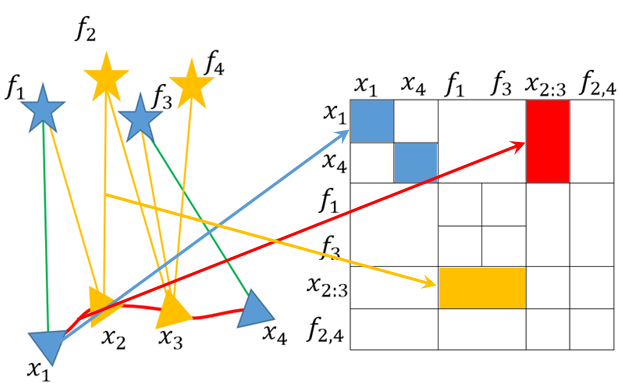
\includegraphics[width=1.00\textwidth]{images/HessianSparsity.png}
	\label{fig:HessianSparsity}
  \caption{Contribution to the hessian matrix of the overall cost by each constraint. Here pose prior has been shown in blue, IMU in red and visual in yellow.}
\end{figure}

In this way if we consider all the constraints the sparsity pattern that we get is shown in figure (\ref{fig:HessianSparsityAllFillUp}).

\begin{figure}[ht]
	\centering
		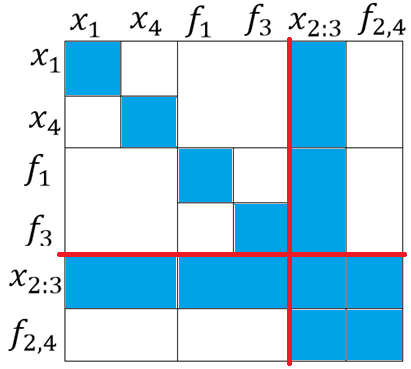
\includegraphics[width=1.00\textwidth]{images/HessianSparsityAllFillUp.png}
	\label{fig:HessianSparsityAllFillUp}
  \caption{Once all the constraints are considered it can be seen that the hessian matrix of BA is inherently sparse. Marginalization of non-key-frame poses cause this sparsity to be lost, if is achieved by taking the Schur complement of the block matrix in second quadrant.}
\end{figure}

As pointed out earlier by comparing figure (\ref{fig:HessianSparsityAllFillUp}) and Eq.(\ref{H_NEW_G_NEW}), it is clear that the marginalized hessian matrix and gradient vector is found by taking the Schur complement of the block matrix that lie in the second quadrant created by the red lines in figure (\ref{fig:HessianSparsityAllFillUp}). Similar is the case for the gradient vector. It is also easy to see that the fill up between $f_1$ and $f_5$ is caused due to our choice of marginalization point, i.e. the place at which we put the red lines in figure (\ref{fig:HessianSparsityAllFillUp}). If we instead place the marginalization point as shown in figure (\ref{fig:HessianSparsityAllFillUpKeepSparsity}), we would make only $x_1\-x_4$ block dense. Since the dimension of this block is very small (in our implementation 12x12), the subsequent optimization would not be impacted in computational cost significantly.

\begin{figure}[ht]
	\centering
		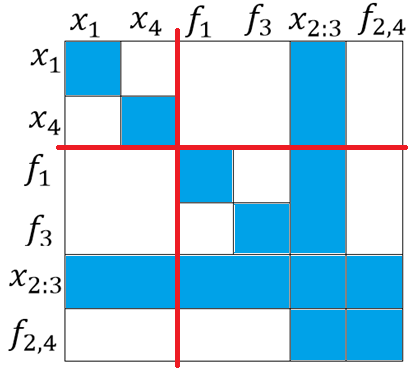
\includegraphics[width=1.00\textwidth]{images/HessianSparsityAllFillUpKeepSparsity.png}
	\label{fig:HessianSparsityAllFillUpKeepSparsity}
  \caption{CKLAM avoids making a substantial part of the hessian matrix dense by marginalizing out the constraints between features seen from key frame and non-key-frame. The effect can be visualized in figure \ref{fig:CKLAMMarginalizationFeatureClone}}
\end{figure}

One point to be noticed here though is that since we marginalized the landmarks $f_1$ and $f_5$ we either should not add an error term corresponding to the constraint represented by $x_1$, $f_1$ observation link while calculating the the hessian matrix, in which case the marginalization will have the effect represented by figure (\ref{fig:CKLAMMarginalizationFeatureClone}), or we should not reuse the $f_1$ landmarks in the batch optimization we used for CKLAM calculation. 

\begin{figure}[ht]
	\centering
		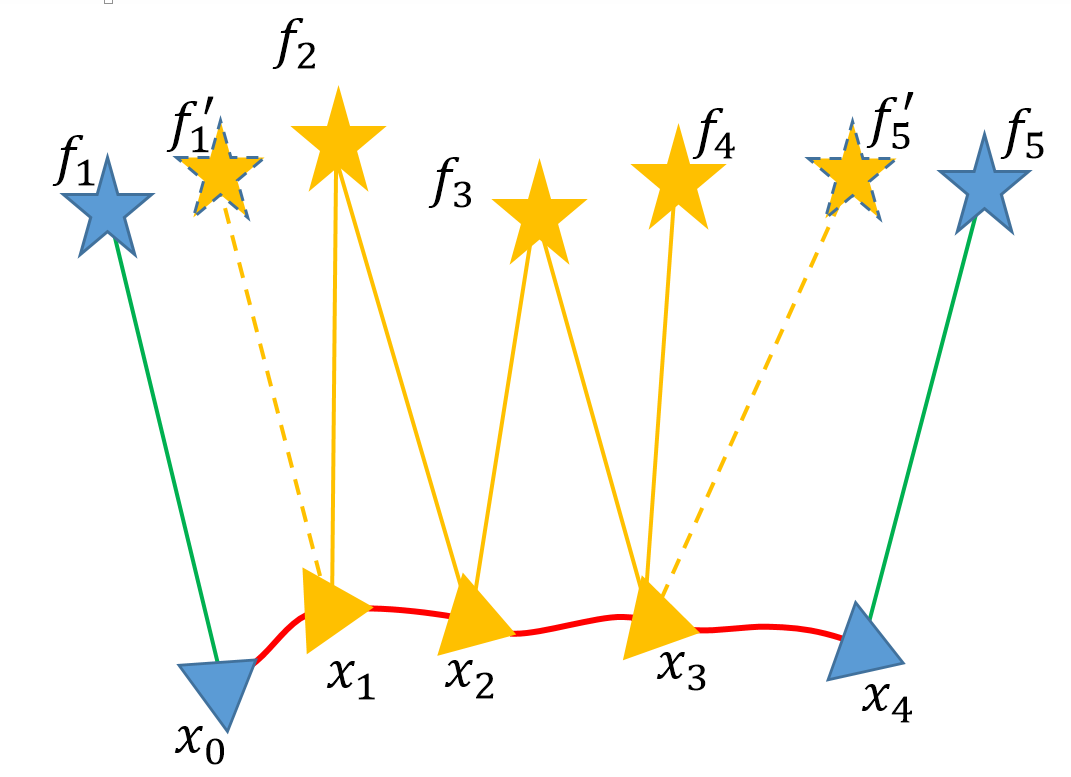
\includegraphics[width=1.00\textwidth]{images/CKLAMMarginalizationFeatureClone.png}
	\label{fig:CKLAMMarginalizationFeatureClone}
  \caption{In order to avoid making the hessian matrix dense CKLAM marginalizes the constraints between non-key-frames and landmarks observed from key-frames. In effect it is as if we had a copy of $f_1$ and $f_5$ that got marginalized, while $f_1$ and $f_5$ were not modified. \cite{CKLAM}}
\end{figure}

A dense information matrix between key frame poses $x_1$ and $x_4$ represents constraints imposed by non key frames on the key frames. In a completely generalized setting where we have prior information about absolute position e.g. when we have GPS information of frames, we can rewrite the batch optimization cost function in Eq.(\ref{BA_FULL_COST}) as in Eq.(\ref{BA_FULL_COST_REWRITTEN})

\begin{equation}
  \begin{split}
    C(x_{0:4},f_{1:5};Z_{0:5},u_{0:3}) = \sum_{i=0}^4 \frac{1}{2}||x_i-\hat x_{i|i}||^2_{P_{i|i}} + \sum_{i=0}^3 {\frac{1}{2}||x_{i+1} - f(x_i, u_i)||^2_{Q_i^{'}}} +\\ \sum_{Z_{ij}\in Z_{0:5}} {\frac{1}{2}||Z_{ij}-h(x_i,f_j)||^2_{R_{ij}}}
    \label{BA_FULL_COST_REWRITTEN}
  \end{split}
\end{equation}

Here $x_i ~ \mathcal{N}(\hat x_{i|i}, P_{i|i})$ represents the prior about the robot poses. The function $f(x_i, u_i)$ represents the propagation function, in our case this function represents the IMU integration function. Finally, $h(x_i,f_j)$ represents measurement function. In our case this function is the camera projection. Following the marginalization methodology discussed above we see that after marginalization the cost function in Eq.(\ref{BA_FULL_COST_REWRITTEN}) is approximated with Eq.(\ref{CKLAM_APPROX})

\begin{equation}
	C_{CKLAM} = \frac{1}{2}
							\begin{bmatrix} 
								x_{1} - \hat x_{1} \\
								x_{2} - \hat x_{2} \\
							\end{bmatrix}^T H_{CKLAM} 
							\begin{bmatrix} 
								x_{1} - \hat x_{1} \\
								x_{2} - \hat x_{2} \\
							\end{bmatrix} + g_{CKLAM}^T
							\begin{bmatrix} 
								x_{1} - \hat x_{1} \\
								x_{2} - \hat x_{2} \\
							\end{bmatrix}
	\label{CKLAM_APPROX}
\end{equation}

\section{CKLAM and Observability of BA}
\label{cklamObservability}
From the form of Eq.(\ref{CKLAM_APPROX}) we see that if $H_\mathrm{new}$ is dense then the information from non key frame poses is represented as Gaussian prior on $\begin{bmatrix} x_{1} \\ x_{2} \end{bmatrix}$, i.e. the key frame poses. This also means that the poses are globally constrained and does not have any free degree of freedom. Since we had absolute priors for the poses e.g. from GPS readings, absolute constraints are explainable and the formulation does not generate false constraints. But often in visual inertial localization and mapping we do not have any absolute position/pose measurement e.g. GPS measurements. In such a situation the prior pose error terms in Eq.(\ref{BA_FULL_COST_REWRITTEN}) i.e. $\sum_{i=0}^4 \frac{1}{2}||x_i-\hat x_{i|i}||^2_{P_{i|i}}$ can not be computed and hence dropped. This causes the whole cost function to have $4$ degrees of freedom (three from absolute position and one due to yaw angle), i.e. the cost function hessian becomes rank deficient by degree $4$. Since the cost function does not constrain all the independent parameters a visual inertial mapping system in absence of external absolute measurement is unobservable. This is the reason for drift corruption of vimaps. In order to get a reasonable solution in absence of absolute measurements, e.g. in case of GPS outage we often fix the first vertex to origin with a prior, with the hope that if an external measurement is made available at a later time we shall move the whole map segment by the given transformation. Now if we go ahead as the previous formulation still, we see that although there exists free degrees of freedom in the batch optimization cost, we create a dense marginalized information matrix. This directly results in creation of false constrains causing the subsequent optimization i.e. optimization with CKLAM to lose these degrees of freedom. Hence the problem becomes over constrained and behave poorly when true information constraining these degrees of freedom are received, e.g. while performing loop closure. Also since after marginalization the information of a CKLAM block is represented in the global frame in which the map segment is represented the calculation has to be re-performed if it a change of frame of reference is required, which is often the case when a place is mapped with multiple agents. To overcome all these difficulties, let us consider a slightly modified version of CKLAM termed Relative-CKLAM in the following chapter. In the relative version of CKLAM we try to marginalize the non-key-frame information as before but represent them with respect to the relative transformation between consecutive key-frames as opposed to directly projecting it onto the key-frame poses.

\chapter{Relative CKLAM}
\label{sec:RCKLAM}

From the discussion in the previous chapter we have seen that CKLAM over constrains the optimization by generating absolute priors to the key frame poses. We argue that it can be avoided if instead of using $\begin{bmatrix} x_{1} \\ x_{2} \end{bmatrix}$ directly as the independent variables to represented the marginalized cost we use a function $R(x_1, x_2)$ to approximate the cost in Eq.(\ref{CKLAM_APPROX}) as given by Eq.(\ref{COST_RCKLAM}). Where $R(x_1, x_2)$ represent the pose of frame $x_2$ with respect to frame $x_1$ in frame $x_1$. 

\begin{equation}
	C = R(x_1, x_2)^TH_\mathrm{RCKLAM}R(x_1, x_2) + g_\mathrm{RCKLAM}^TR(x_1, x_2)
	\label{COST_RCKLAM}
\end{equation}
This claim is based on the observation we made in section \ref{cklamObservability}. There we identified that the root cause of over-constraining nature of CKLAM lies in its way of representation of non-key-frame information. Since non-key-frames link the key frames it is natural to summarize their contribution as a relative transformation. This underpins the objective of RCKLAM. Given the information about the non-key-frames we would like to compute the mean value along with its covariance of relative transformation between two key frames. The corresponding quantities are represented here by $R(x_1, x_2)$, $H_\mathrm{RCKLAM}$ and $g_\mathrm{RCKLAM}$
Clearly we now have to calculate $H_\mathrm{RCKLAM}$ from the full batch cost given by Eq.(\ref{BA_FULL_COST_REWRITTEN}). We shall do it in two steps. First, we shall take the the CKLAM cost function given by Eq.(\ref{CKLAM_APPROX}) and then modify the hessian matrix and the gradient vector of it to generate $H_\mathrm{RCKLAM}$ and $g_\mathrm{RCKLAM}$.

\section{RCKLAM expectation}
\label{sec:RCKLAMExpectation}
In this section let us formalize the expected behavior of RCKLAM so we can compare it against the obtained results. As discussed in the previous sections, we expect RCKLAM to better represent the information from non key frames by keeping distribution of integrated noise as is while by projecting them onto the individual poses CKLAM transforms them to individual Gaussian fixed in a global frame and hence canot efficiently propaget new information through out ht emap efficiently. This situation is most prominent in case of loo closure, especially when loop closere happen after a long time and with a large drift. Let us consider a hypothetical situation as in figure \ref{fig:hypotheticalLoopClosure}
\begin{figure}
	\centering
		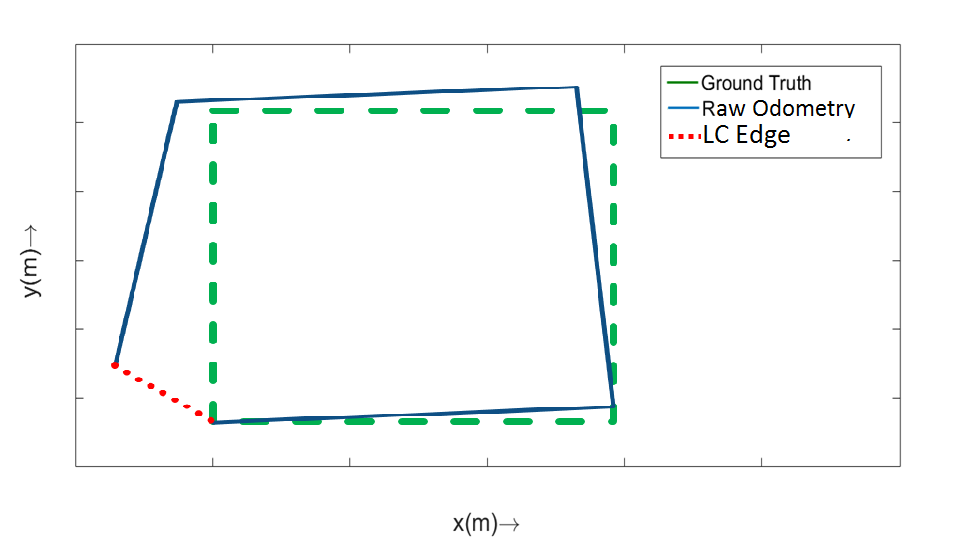
\includegraphics[width=1.00\textwidth]{images/hypotheticalLoopClosure.png}
	\label{fig:hypotheticalLoopClosure}
  \caption{Loop closure on a hypothetical rectangular map. Notice that the estimation from the raw odometry is drifting. We are interested in comparing the optimized map with RCKLAM and CKLAM technique. The red edge represent a loop closure edge.}
\end{figure}
Since the loop closure edge now will cause the last vertex to move towards its true position we expect the optimized maps to improve form their first estimate. Yet due to the way of CKLAM's representation we expect it to not propagate the information many vertex back while we expect RCKLAM to achieve better result. Our expectation is summarized in figure \ref{fig:hypotheticalLoopClosureCklamRcklam}
\begin{figure}
	\centering
		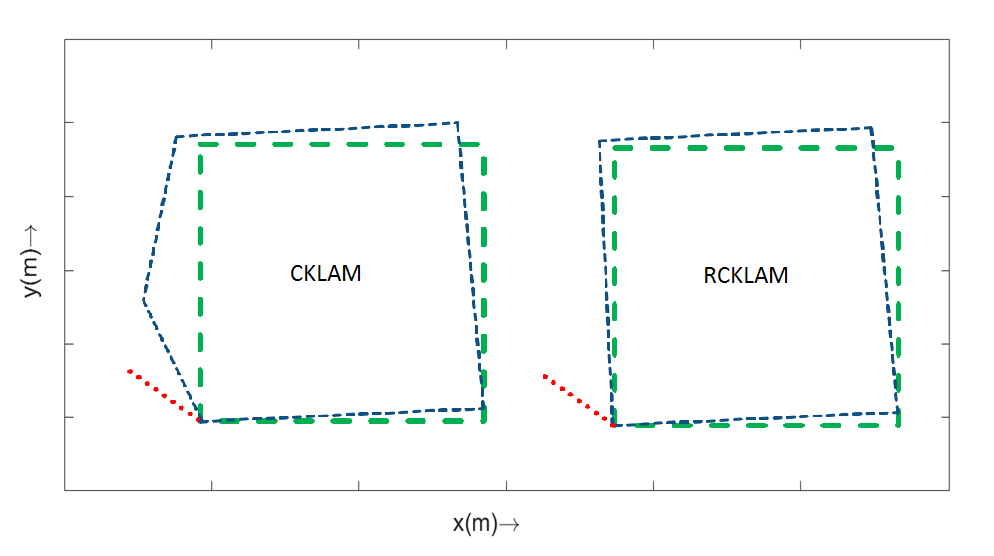
\includegraphics[width=1.00\textwidth]{images/hypotheticalLoopClosureCklamRcklam.png}
	\label{fig:hypotheticalLoopClosureCklamRcklam}
  \caption{From the discussion in section \ref{sec:RCKLAMExpectation} here we summarize the expected optimization result with CKLAM and RCKLAM. We expect that CKLAM will limit the information propagation while RCKLAM will not do so. This claim is verified by the result shown in figure \ref{fig:Syn16MapLoppClosureSym}}
\end{figure}

 

\section{RCKLAM Formulation}
\label{rcklamSimple}
For simplicity, let us momentarily assume that the pose of frame $x_2$ in frame $x_1$ with respect to $x_1$ is given by the simple  subtraction operation, i.e. $R(x_1, x_2) = x_2 - x_1$. Once we have established the methodology we shall look at the generalized case of it with a non linear function $R$ so as to deal with inverse quaternion multiplication. Given the cost function in Eq.(\ref{CKLAM_APPROX}) we wish to re-write it as in Eq.(\ref{CKLAM_COST_REWRITTEN})

\begin{equation}
	C = \begin{bmatrix} x_1-x_2 \\ x_2 \end{bmatrix} ^TH_1\begin{bmatrix} x_1-x_2 \\ x_2 \end{bmatrix} + g_1^T\begin{bmatrix} x_1-x_2 \\ x_2 \end{bmatrix}
	\label{CKLAM_COST_REWRITTEN}
\end{equation}

Clearly $\begin{bmatrix} x_1-x_2 \\ x_2 \end{bmatrix}$ can be written as $\begin{bmatrix} 1 & -1\\ 0 & 1\end{bmatrix} \begin{bmatrix} x_1-x_2 \\ x_2 \end{bmatrix}$. Replacing these results into Eq.(\ref{CKLAM_COST_REWRITTEN}) gives it the form as given by Eq.(\ref{rcklamSimple_CASE})

\begin{equation}
	C = \begin{bmatrix} x_1 \\ x_2 \end{bmatrix} ^T\begin{bmatrix} 1 & -1\\ 1 & 0 \end{bmatrix}^T H_1\begin{bmatrix} 1 & -1\\ 1 & 0 \end{bmatrix} \begin{bmatrix} x_1 \\ x_2 \end{bmatrix} + g_1^T\begin{bmatrix} 1 & -1\\ 1 & 0 \end{bmatrix}\begin{bmatrix} x_1 \\ x_2 \end{bmatrix}
	\label{rcklamSimple_CASE}
\end{equation}

Comparing Eq.(\ref{CKLAM_APPROX}) and Eq.(\ref{rcklamSimple_CASE}) we can draw the relationship between the CKLAM hessian matrix and $H_1$, similar is the case with the gradient vectors. The relationship is as given in Eq.(\ref{RCKLAM_FROM_CKLAM}) 

\begin{subequations}
	\begin{equation}
		H_\mathrm{CKLAM} = \begin{bmatrix} 1 & -1\\ 1 & 0 \end{bmatrix}^T H_1\begin{bmatrix} 1 & -1\\ 1 & 0 \end{bmatrix}
	\end{equation}
	\begin{equation}
		g_\mathrm{CKLAM} = g_1\begin{bmatrix} 1 & -1\\ 1 & 0 \end{bmatrix}
	\end{equation}
	\label{RCKLAM_FROM_CKLAM}
\end{subequations}

Clearly we still do not have the form of the cost function as given in Eq.(\ref{COST_RCKLAM}), which is necessary for RCKLAM, but it can be recognized easily that it is very similar to the CKLAM problem we had in the beginning. Just like before once again we have a function of two variables and we would like to eliminate one of them. So once more we deploy Schur complement technique to eliminate the independent variable, $x_2$ in this case.

\section{RCKLAM Generalized Relative Pose Computation}
However our assumption that finding relative pose between two consecutive poses is linear operation, i.e. $R(x_1, x_2) = x_2 - x_1$, does not hold true once the pose representation contain quaternions for orientation since inverse quaternion multiplication is not a linear operation. So we would like to follow a general derivation similar to the one described in section \ref{rcklamSimple}. Eventually we shall find a similar relation ship as in Eq.(\ref{RCKLAM_FROM_CKLAM}) when linearity of $R(x_1, x_2)$ is not assumed and is considered a general nonlinear but differentiable function. Let us start with Eq.(\ref{CKLAM_APPROX}) and as before the objective would be to find the relationship of the hessian matrix and the gradient vector of it to the ones in Eq.(\ref{COST_RCKLAM}). As we can only represent linear operations through matrix manipulation we linearize $R$ by Taylor expansion. This is given by Eq.(\ref{RCKLAM_LINEAR_COST})

\begin{equation}
  R(x_1, x_2) \approx R(\hat x_1, \hat x_2) + \frac{\partial R} {\partial x_1}\biggr\rvert_{\hat x_1, \hat x_2} (x_1 - \hat x_1)+ \frac{\partial R} {\partial x_2}\biggr\rvert_{\hat x_1, \hat x_2} (x_2 - \hat x_2)
	\label{RCKLAM_LINEAR_COST}
\end{equation}

In order to simplify the calculation let us reformulate the cost function as follows
\begin{equation}
  \begin{split}
    C = \frac{1}{2}R(x_1, x_2)^TH_\mathrm{RCKLAM}R(x_1, x_2) + g_\mathrm{RCKLAM}^TR(x_1, x_2) = \\ (A_\mathrm{RCKLAM}R(x_1, x_2) + b_\mathrm{RCKLAM})^T(A_\mathrm{RCKLAM}R(x_1, x_2) + b_\mathrm{RCKLAM})
    \label{COST_RCKLAM_FACTORIZED}
    \end{split}
\end{equation}
 Where $A^TA = \frac{1}{2}H_\mathrm{CKLAM}$ and $b = \frac{1}{2} A^{-T}g$. Since there is a direct inexpensive way to calculate $A$ and $b$ and the square root cost $AR(x_1, x_2) + b$ is easier to manipulate, we redefine the objective as the follows. Instead of trying to find an equivalent $H_\mathrm{RCKLAM}$ and $g_\mathrm{RCKLAM}$ we would now find $A_\mathrm{RCKLAM}$ and $b_\mathrm{RCKLAM}$ such that the square root cost is equivalent. The objective is formalized in Eq.(\ref{RCKLAM_OBJECTIVE})

\begin{equation}
  C_\mathrm{sqrt} = A_\mathrm{CKLAM}\begin{bmatrix} x_1 \\ x_2 \end{bmatrix} + b_\mathrm{CKLAM}\approx A_\mathrm{RCKLAM}R(x_1, x_2) + b_\mathrm{RCKLAM}
	\label{RCKLAM_OBJECTIVE}
\end{equation}
But before attempting to find $A_\mathrm{RCKLAM}$ and $b_\mathrm{RCKLAM}$, we will calculate get $A_1$ nad $b_1$ such that :
\begin{equation}
  C_\mathrm{sqrt} = A_1\begin{bmatrix} R(x_1, x_2) \\ x_2 \end{bmatrix} + b_1
	\label{RCKLAM_OBJECTIVE_derivation0}
\end{equation}
Replacing the linear approximation of function $R$ in the right hand side of Eq.(\ref{RCKLAM_OBJECTIVE_derivation0}) we get : 
\begin{equation}
  C_\mathrm{sqrt}\approx A_1\begin{bmatrix} R(\hat x_1, \hat x_2) + j_1(x_1 - \hat x_1) + j_2(x_2 - \hat x_2) \\ x_2 \end{bmatrix} + b_1
  \label{RCKLAM_OBJECTIVE_derivation1}
\end{equation}
Where $j_1 = \frac{\partial R}{\partial x_1}\biggr\rvert_{\hat x_1, \hat x_2}$ and $j_2 = \frac{\partial R}{\partial x_2}\biggr\rvert_{\hat x_1, \hat x_2}$. Let $R(\hat x_1, \hat x_2) - j_1\hat x_1 - j_2\hat x_2 = \alpha$, then Eq.(\ref{RCKLAM_OBJECTIVE_derivation1}) becomes :
\begin{equation}
  C_\mathrm{sqrt}\approx A_1\begin{bmatrix} \alpha + j_1x_1 + j_2x_2 \\ x_2 \end{bmatrix} + b_1
  \label{RCKLAM_OBJECTIVE_derivation2}
\end{equation}
Factoring out $\alpha$ with distribution of multiplication over addition we get :
\begin{equation}
  C_\mathrm{sqrt}\approx A_1\begin{bmatrix} j_1x_1 + j_2x_2 \\ x_2 \end{bmatrix} + A_1\begin{bmatrix}\alpha \\ 0\end{bmatrix}b_1
  \label{RCKLAM_OBJECTIVE_derivation3}
\end{equation}
Eq.(\ref{RCKLAM_OBJECTIVE_derivation3}) can further be rewritten as :
\begin{equation}
  C_\mathrm{sqrt}\approx A_1\begin{bmatrix}j_1 & j_2 \\ 0 & 1\end{bmatrix}\begin{bmatrix} x_1 \\ x_2 \end{bmatrix} + A_1\begin{bmatrix}\alpha \\ 0\end{bmatrix} + b_1
  \label{RCKLAM_OBJECTIVE_derivation4}
\end{equation}
Eq.(\ref{RCKLAM_OBJECTIVE_derivation4}) can now directly be compared with Eq.(\ref{RCKLAM_OBJECTIVE}) to get $A_1\begin{bmatrix}j_1 & j_2 \\ 0 & 1\end{bmatrix} = A_\mathrm{CKLAM}$ and $A_1\begin{bmatrix}\alpha \\ 0\end{bmatrix} + b_1 = b_\mathrm{CKLAM}$. From these results it is trivial to compute $A_1$ and $b_1$ given $A_\mathrm{CKALM} , b_\mathrm{CKLAM}$. This is given by Eq.(\ref{A_1b_1CALC})

\begin{subequations}
  \begin{equation}
    A_1 = A_\mathrm{CKALM}\begin{bmatrix}j_1 & j_2 \\ 0 & 1\end{bmatrix}^{-1}
  \end{equation}
  \begin{equation}
    b_1 = b_\mathrm{CKLAM} - A_1 \begin{bmatrix}\alpha \\ 0 \end{bmatrix}
  \end{equation}
  \label{A_1b_1CALC}
\end{subequations}
In order to find the relationship betwen $A_1$ and $A_\mathrm{RCKLAM}$ we have to marginalize out the independent variable $x_2$, as we did before while developing the CKLAM hessian as well as while deriving the RCKLAM hessian for the simple case. One point to be noticed here is that, since here we have the square root of the cost function we do not have the hessian matrix itself but $A$ which satisfies $A^TA = \frac{1}{2}H$. Similar is the case for the gradient vector. But as can be seen from Appendix-\ref{sec:schur_sqrt_cost} we can still take the Schure complement to eliminate $x_2$ in exactly the same way as in chapter \ref{sec:CKLAM}.


\chapter{Experimental Results}
\label{chap:ExptAndResults}
  In this chapter we shall represent the experiment results obtained with the simulation and real-life data. We shall first present the simulation result to validate the expectations we put forward in the previous chapters, especially the advantage we expect to gain by RCKLAM framework. The simulation maps were kept simple for easier visualization and to avoid complexity.
  
\section{Experimentation in Simulation}
\label{sec:SimulationExpt}

  In figure \ref{fig:Syn31Map} we assume that the sliding window estimator is unable to recover the true camera poses and generates a map which deviates for the true map in a random way. The corrupted map is represented by red line while the true map is represented in green line.
  
  
\begin{figure}
  \centering
    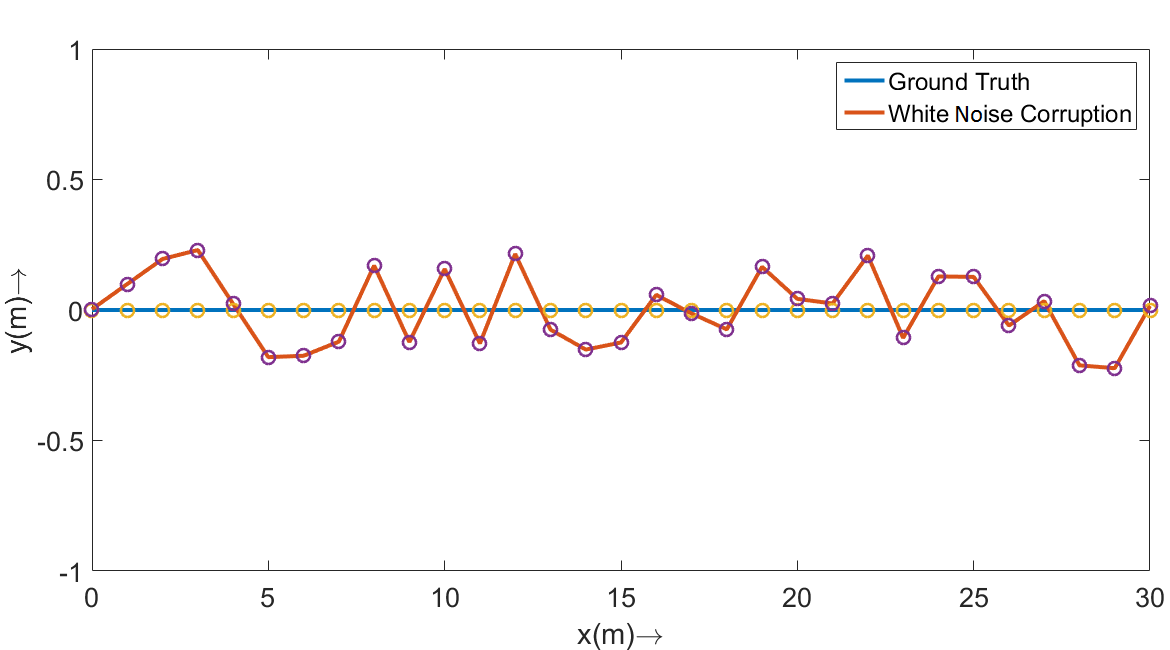
\includegraphics[width=1.00\textwidth]{images/Syn31_map.png}
  \label{fig:Syn31Map}
  \caption{Ground truth and simulated sliding window estimation. Ground truth given by green line and simulated odometry result given by red line. This is a low bias high variance situation so the estimator is simulated as drift free. This experiment measures CKLAM and RCKLAM's noise tolerance.}
\end{figure}
  
  
  The corrupted map is then optimized with both CKLAM and full batch optimization technique. Figure \ref{fig:Syn31ErrorPlotCKLAM} shows the error norm against vertex index obtained by both of these methods. Clearly both of the optimizations improve the results and CKLAM is fairly close to the full batch optimization method. 
  
  
\begin{figure}
  \centering
    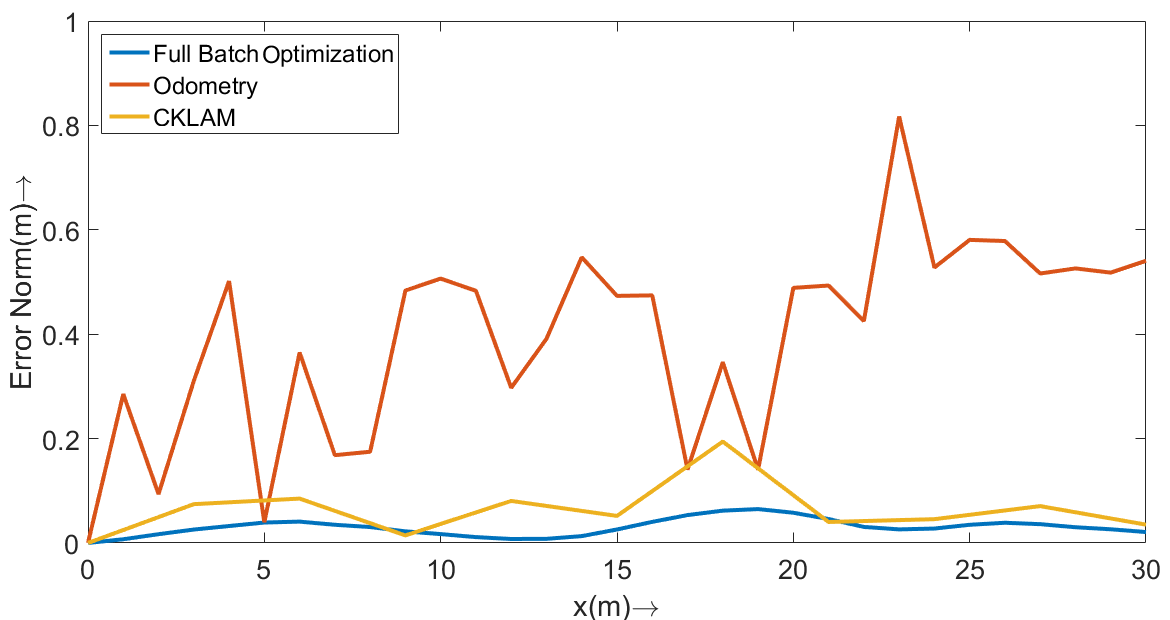
\includegraphics[width=1.00\textwidth]{images/Syn31_error_plot_CKLAM.png}
  \label{fig:Syn31ErrorPlotCKLAM}
  \caption{Performance of CKLAM compared against full batch optimization starting with low bias high variance noise corrupted map.}
\end{figure}
  
  
  Figure \ref{fig:Syn31ErrorPlot} shows the results of the same experiment except for the introduction of RCKLAM. The error norm given by RCKLAM is given in purple line. Clearly RCKLAM matches closely CKLAM in terms of optimization quality.
    
  \begin{figure}
    \centering
      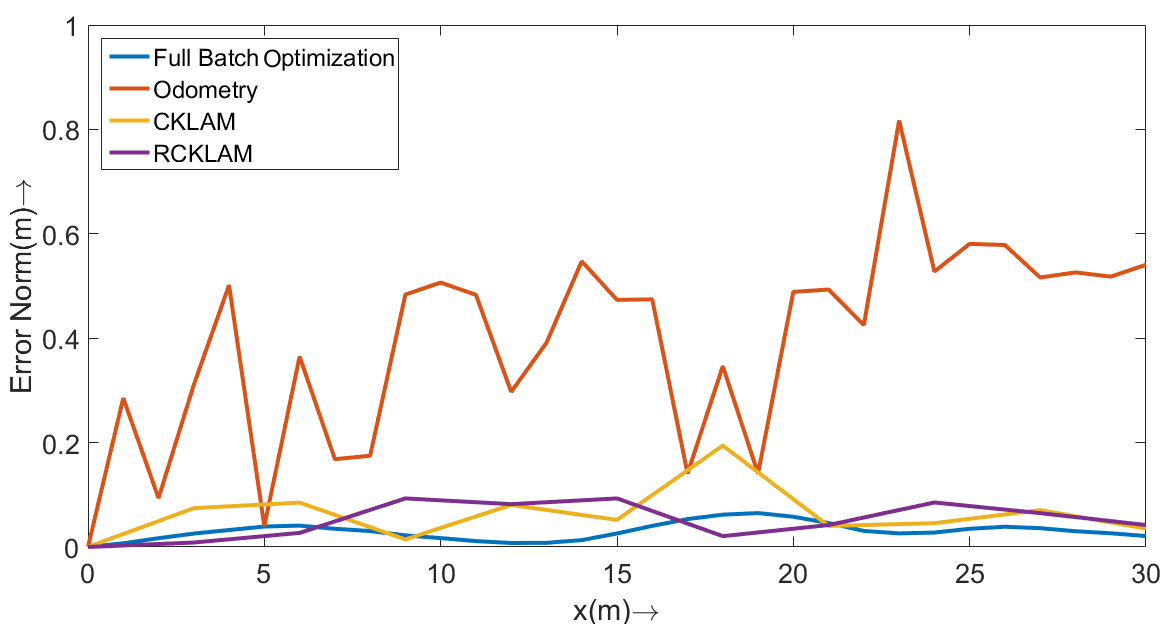
\includegraphics[width=1.00\textwidth]{images/Syn31_error_plot.png}
    \label{fig:Syn31ErrorPlot}
    \caption{Performance of RCKLAM compared against full batch optimization and CKALM starting with low bias high variance noise corrupted map.}
  \end{figure}
  
  To verify the claim of section \ref{sec:RCKLAM} with the help of figure \ref{sec:RCKLAMExpectation}, we simulated a map in which the camera translates in $x$ direction with constant velocity and simulate a drifting sliding window estimator. In this simulation experiment the camera drifts in the positive $Y$ direction, and finally we optimized the drifted map with CKLAM technique. To create a reference point of CKLAM's performance in presence of drift corruption we simulated CKLAM optimization first without loop closure. The results of this experiment is shown in figure \ref{fig:Syn16MapCklam} the ground truth map is given in red line while the drift corruption map is given in purple line, and finally the sky blue line represents the optimized map given by CKLAM. An important point to be noticed here is that unlike the previous methods where we plotted error norm with respect to vertex index, here we plot the vertex positions themselves. It is clear that although the quality has improved the optimized map still depicts drift error and confirms our expectation that CKLAM might perform poorly in case of presence of loop closure edge since it binds the key frames in global frame.
  
\begin{figure}
  \centering
    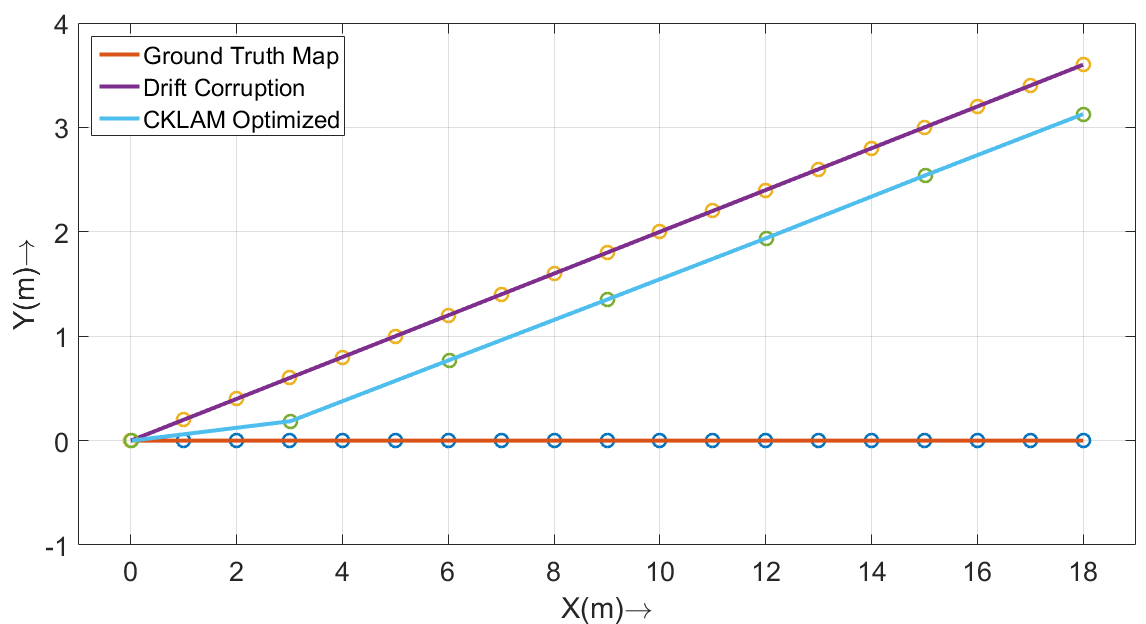
\includegraphics[width=1.00\textwidth]{images/Syn16_map_cklam.png}
  \label{fig:Syn16MapCklam}
  \caption{Performance of CKLAM starting with high bias low variance noise corrupted map. Notice that although CKALM optimization improves from the starting position because of unobservability of absolute position the result is also drift corrupted, i.e. the error is allowed to grow without limit given a long enough map.}
\end{figure}
  
  Given the comparison point of CKLAM's performance with drift corrupted map in figure \ref{fig:Syn16MapCklam}, we can now compare the performance of CKLAM against RCKLAM in case of loop closure. To simulate loop closure we add a prior to the last vertex of the drift corrupted map. The mean of the prior is taken from the ground truth value. The result obtained after optimization with both CKALM and RCKLAM is shown in the figure \ref{fig:Syn16MapLoppClosureSym}
  
\begin{figure}[ht]
  \centering
    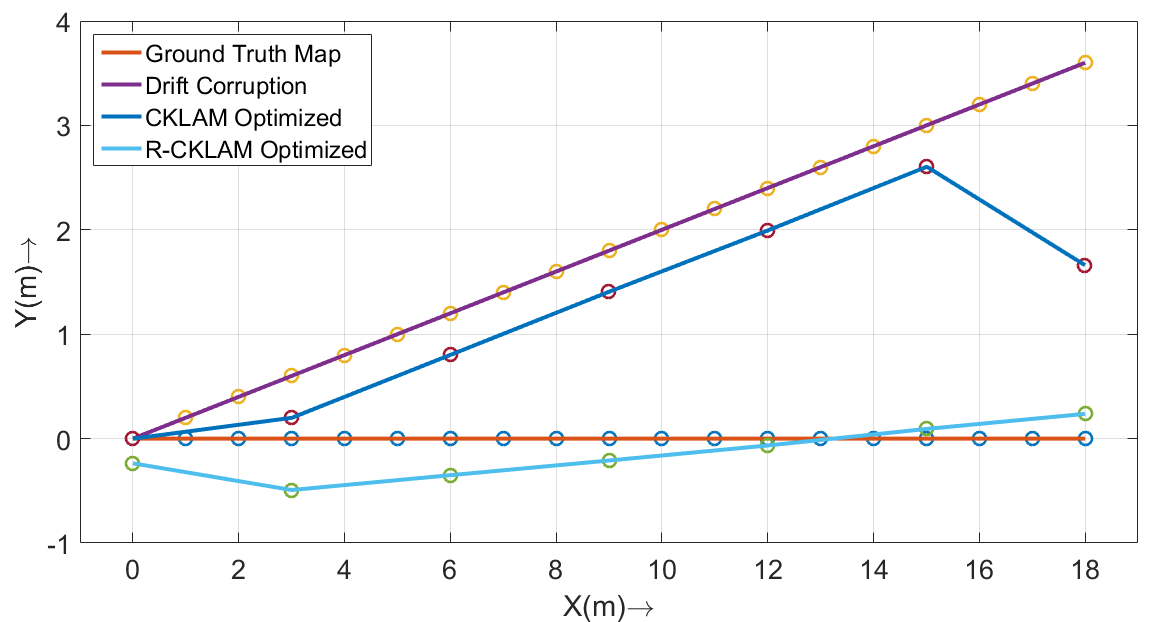
\includegraphics[width=1.00\textwidth]{images/Syn16_map_loppClosureSym.png}
  \label{fig:Syn16MapLoppClosureSym}
  \caption{Simulated loop closure for a high bias corrupted map. Because of CKLAMs design it can not propagate new information well, while RCKLAM efficiently distributes this new information well. The loop closure is simulated by introducing a pose prior to the last vertex.}
\end{figure}

As can be seen from figure \ref{fig:Syn16MapLoppClosureSym} RCKLAM has distributed the loop closing information over the map better than CKLAM as expected. Since RCKLAM only constrains the relative pose between two consecutive key frames, integrated noise is represented as integrated noise. All visual inertial mapping systems underestimates the uncertainty in the estimated poses and RCKLAM is not an exception to that, it is better off as compared to the CKALM, which is evident from figure \ref{fig:Syn16MapLoppClosureSym}. Now we shall have look at the performance of RCKLAM in real-life data.

\section{Experiment With Real life Data}
\label{sec:RealLifeExpt}

The experimental setup consisted of the VI\_sensor \cite{6906892} developed by the Autonomous Systems Lab, ETH and Skybotics. This sensor provides time-synchronized and pre-calibrated inertial measurement unit (IMU) and stereo-camera data streams. The IMU data was recorded at $200$ HZ while the camera frame rate was $20$ HZ. The experement was conducted with the publicly available EuRoC \cite{Burri25012016} dataset. The experiments were done in three different maps with different time duration and complexity levels. The three different mapse were named as MH\_01 through MH\_03. In case of both CKLAM and RCKALM implementation the key frames were selected completely independently. The decision to make a frame, key frame was made by the frame selection algorithm which tried to maintained certain number of common landmarks between consecutive key frames, maintain a maximum distance between key frames and also maintain a certain a maximum rotation angle between key frames. This key framing technique was deployed in order to avoid unconstrained optimization problems in case of aggressive maneuvers. Once the key frames IDs were received the CKLAM algorithm was run to marginalize non-keyframes between them. We compare the performance of CKLAM and RCKLAM with respect to full batch optimization [Bundle Adjustment (BA)], traditional key framing approach and ground truth. In traditional key framing the non-keyframes were simply deleted. Figure \ref{fig:CKLAMvsGT} shows comparison between traditional key framing approach and CKLAM method. Clearly the green line is closer to the blue line as compared to the red one, showing that preserving information from the non-keyframes result in much less error in the resulting map.

\begin{figure}
	\centering
		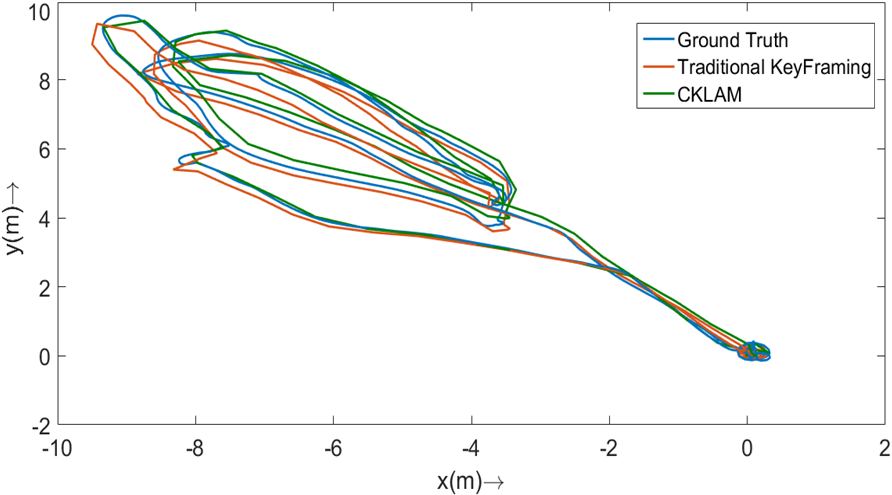
\includegraphics[width=1.00\textwidth]{images/CKLAMvsGT.png}
	\label{fig:CKLAMvsGT}
  \caption{Data set MH\_02 from EuRoC \cite{Burri25012016} data set collection. Comparison between ground truth (blue), CKLAM(green) and traditional key framing technique(red). Clearly CKLAM by preserving information from non-key-frames perform better than traditional key-framing approach.}
\end{figure}

Figure \ref{fig:RCKLAMvsGT} shows the same experiment repeated with RCKALM in place of CKLAM. Once again the green map is closer to the blue one as compared to the red showing that RCKLAM achieves results superior to traditional key framing. 

\begin{figure}
	\centering
		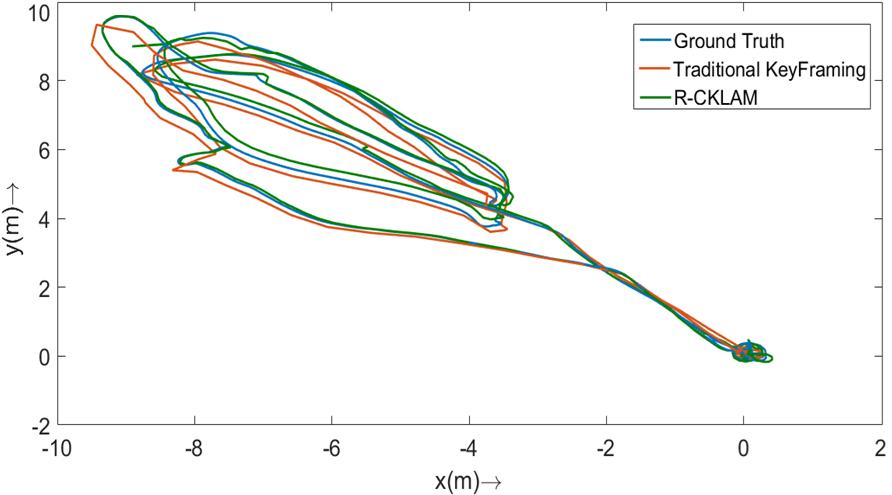
\includegraphics[width=1.00\textwidth]{images/RCKLAMvsGT.png}
	\label{fig:RCKLAMvsGT}
  \caption{Data set MH\_02 from EuRoC \cite{Burri25012016} data set collection. Comparison between ground truth (blue), RCKLAM(green) and traditional key framing technique(red). Clearly RCKLAM by preserving information from non-key-frames perform better than traditional key-framing approach.}
\end{figure}


Since it is difficult to compare more that two methods with the kind of plots represented in the figure \ref{fig:CKLAMvsGT} and figure \ref{fig:RCKLAMvsGT}, let us compare the methods by the mean norm error and variance in that achieved by different methods over an entire map. In order to achieve statistical significance we shall perform this evaluation on multiple maps. Figure \ref{fig:MethodComparisonMH01} through \ref{fig:MethodComparisonMH03} represent the mean error of the vertices optimized with different methods over different maps. We can see that both RCKLAM and CKALM achieve significantly better quality as compared to either the odometry filter or traditional key framing approach, but since we incorporate quadratization error in case of both CKLAM and RCKALM, they perform slightly poorly as compared to the full batch optimization.  

\begin{figure}
	\centering
		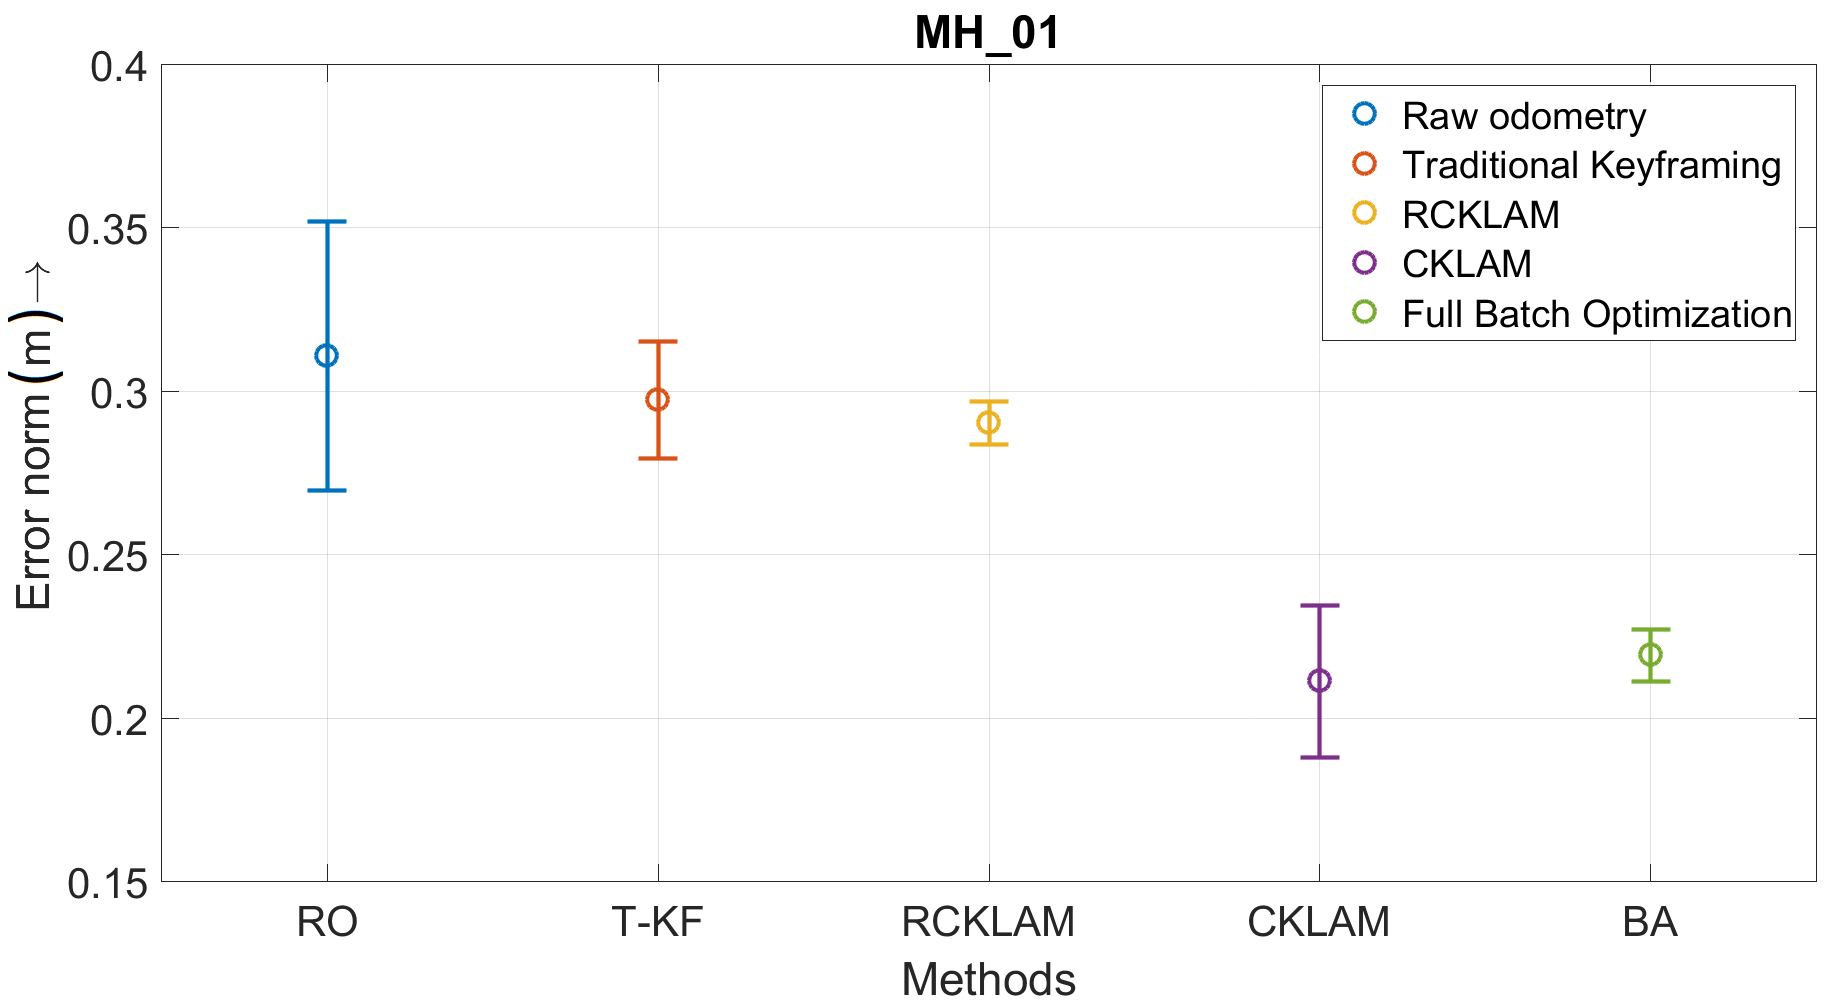
\includegraphics[width=1.00\textwidth]{images/MethodComparisonMH01.png}
	\label{fig:MethodComparisonMH01}
  \caption{Data set MH\_01 from EuRoC \cite{Burri25012016} data set collection. Overall performance quality of different methods on different maps. The average error in every vertex position and their covariance for different methods are represented here.}
\end{figure}

\begin{figure}
	\centering
		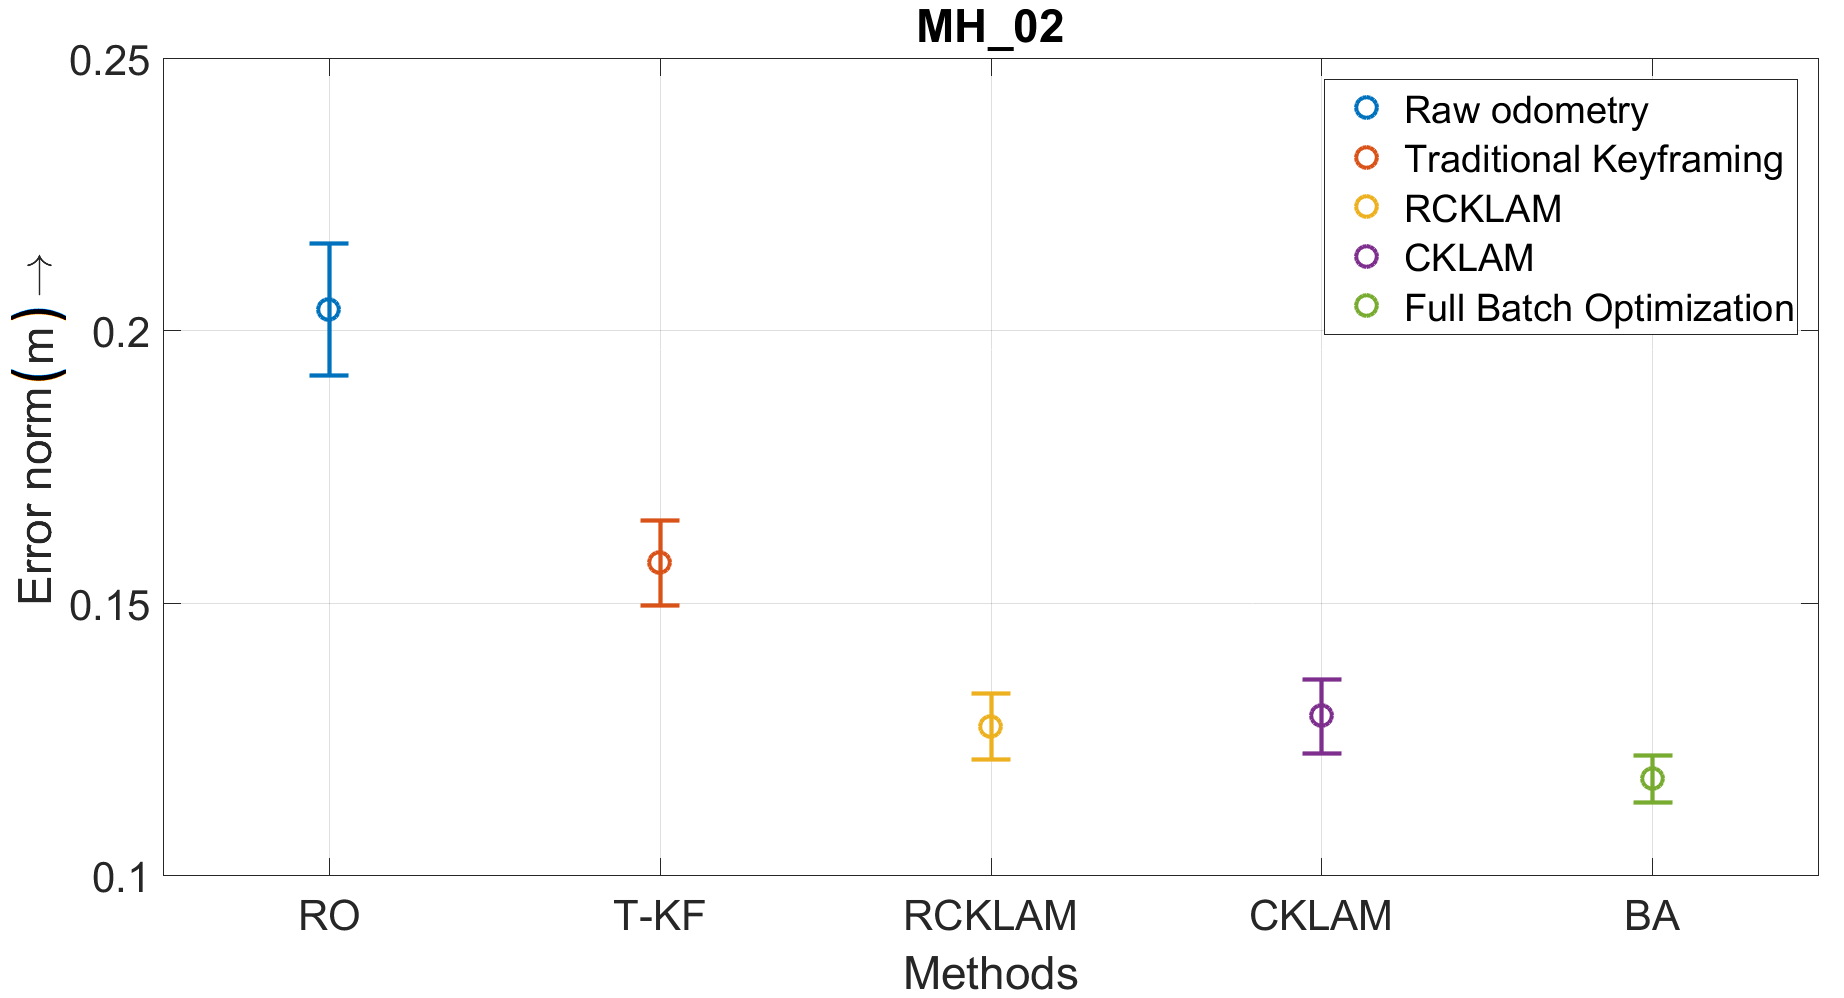
\includegraphics[width=1.00\textwidth]{images/MethodComparisonMH02.png}
	\label{fig:MethodComparisonMH02}
  \caption{Data set MH\_02 from EuRoC \cite{Burri25012016} data set collection. Same experiment as in figure \ref{fig:MethodComparisonMH01}, but with a different data set.}
\end{figure}

\begin{figure}
	\centering
		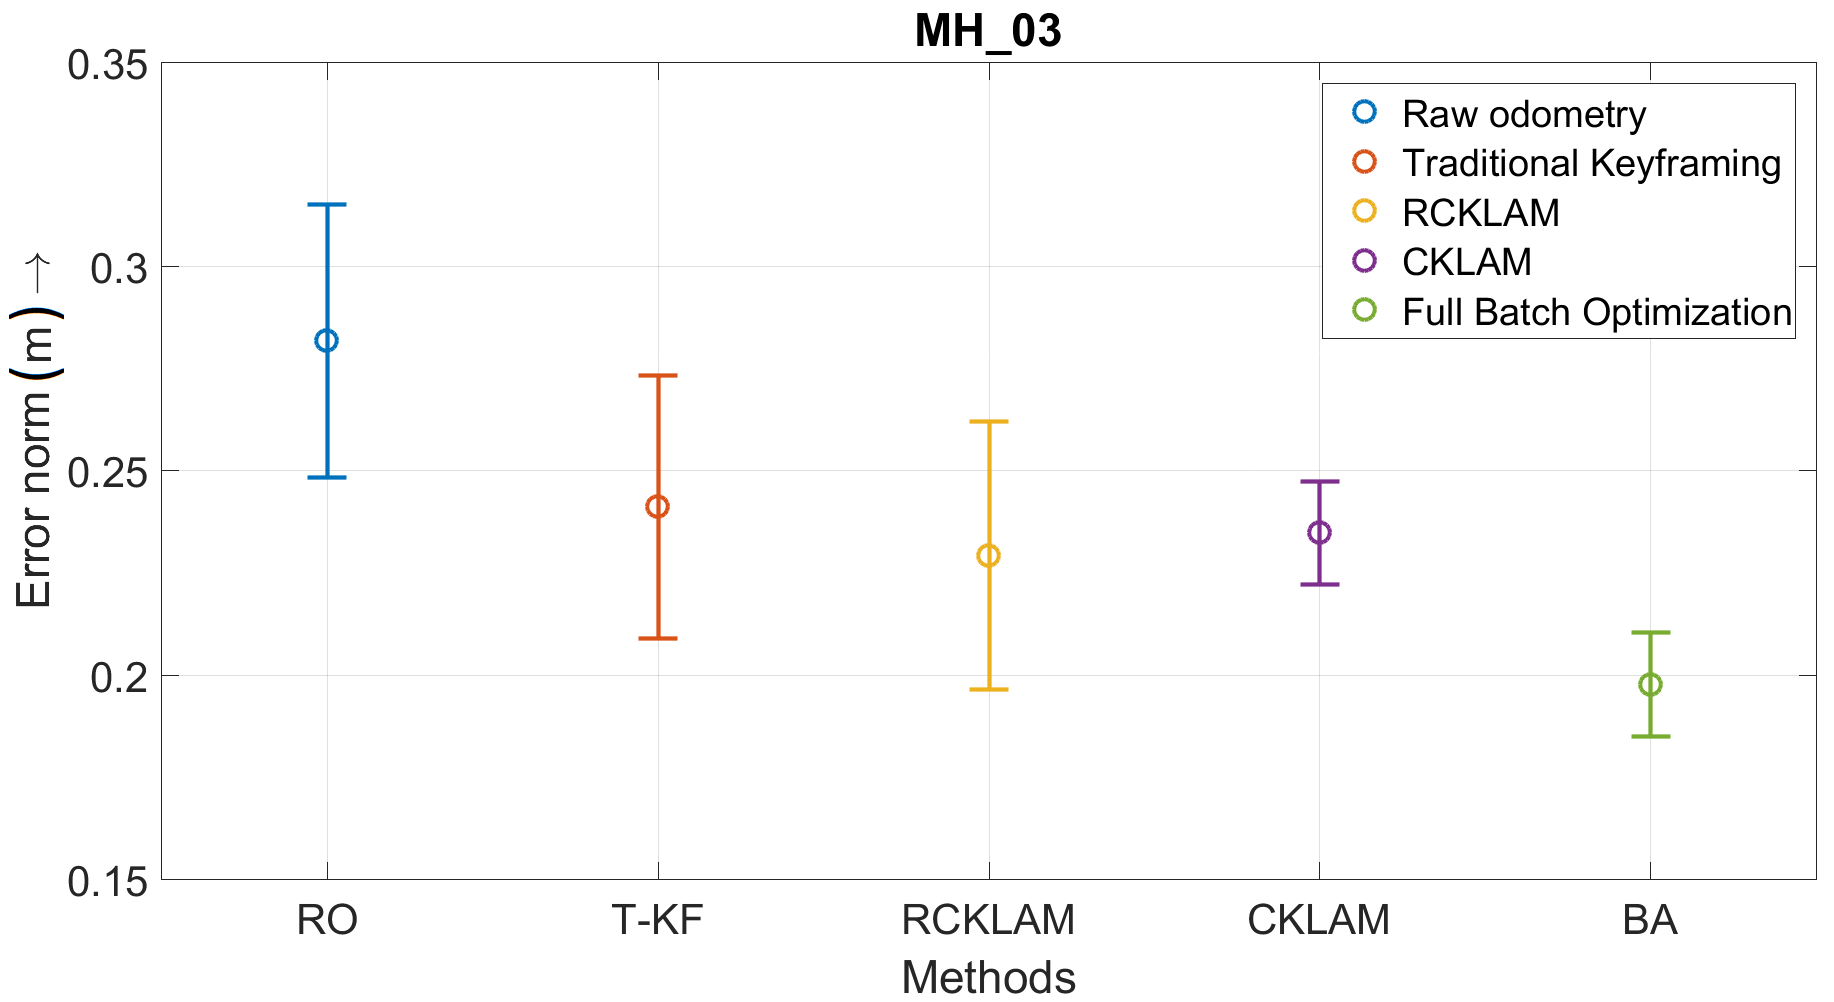
\includegraphics[width=1.00\textwidth]{images/MethodComparisonMH03.png}
	\label{fig:MethodComparisonMH03}
  \caption{Data set MH\_03 from EuRoC \cite{Burri25012016} data set collection. Same experiment as in figure \ref{fig:MethodComparisonMH01}, but with yet another data set.}
\end{figure}

This can be considered as the price we pay for the increase in speed that is achieved. The comparison of computational time requirement for different methods for different maps is shown in figure \ref{fig:MethodComparisonTimeMH01} through \ref{fig:MethodComparisonTimeMH03}. It can easily be noticed that the we gain sizable gain in computational complexity as compared to the full batch optimization, which is often infeasible for large maps. 

\begin{figure}
	\centering
		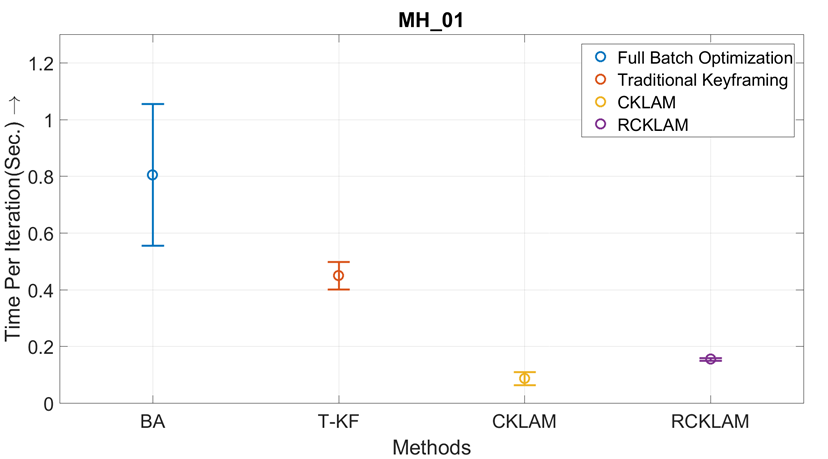
\includegraphics[width=1.00\textwidth]{images/MethodComparisonTimeMH01.png}
	\label{fig:MethodComparisonTimeMH01}
  \caption{Data set MH\_01 from EuRoC \cite{Burri25012016} data set collection. Computational complexity comparison of different methods. Mean time taken of one optimization step for each method and their variance ha been plotted. In this map 122 frames were selected as key-frames out of 913 vertices. The reduction in number of parameters is the main contributor towards the reduction in computational complexity.}
\end{figure}

\begin{figure}
	\centering
		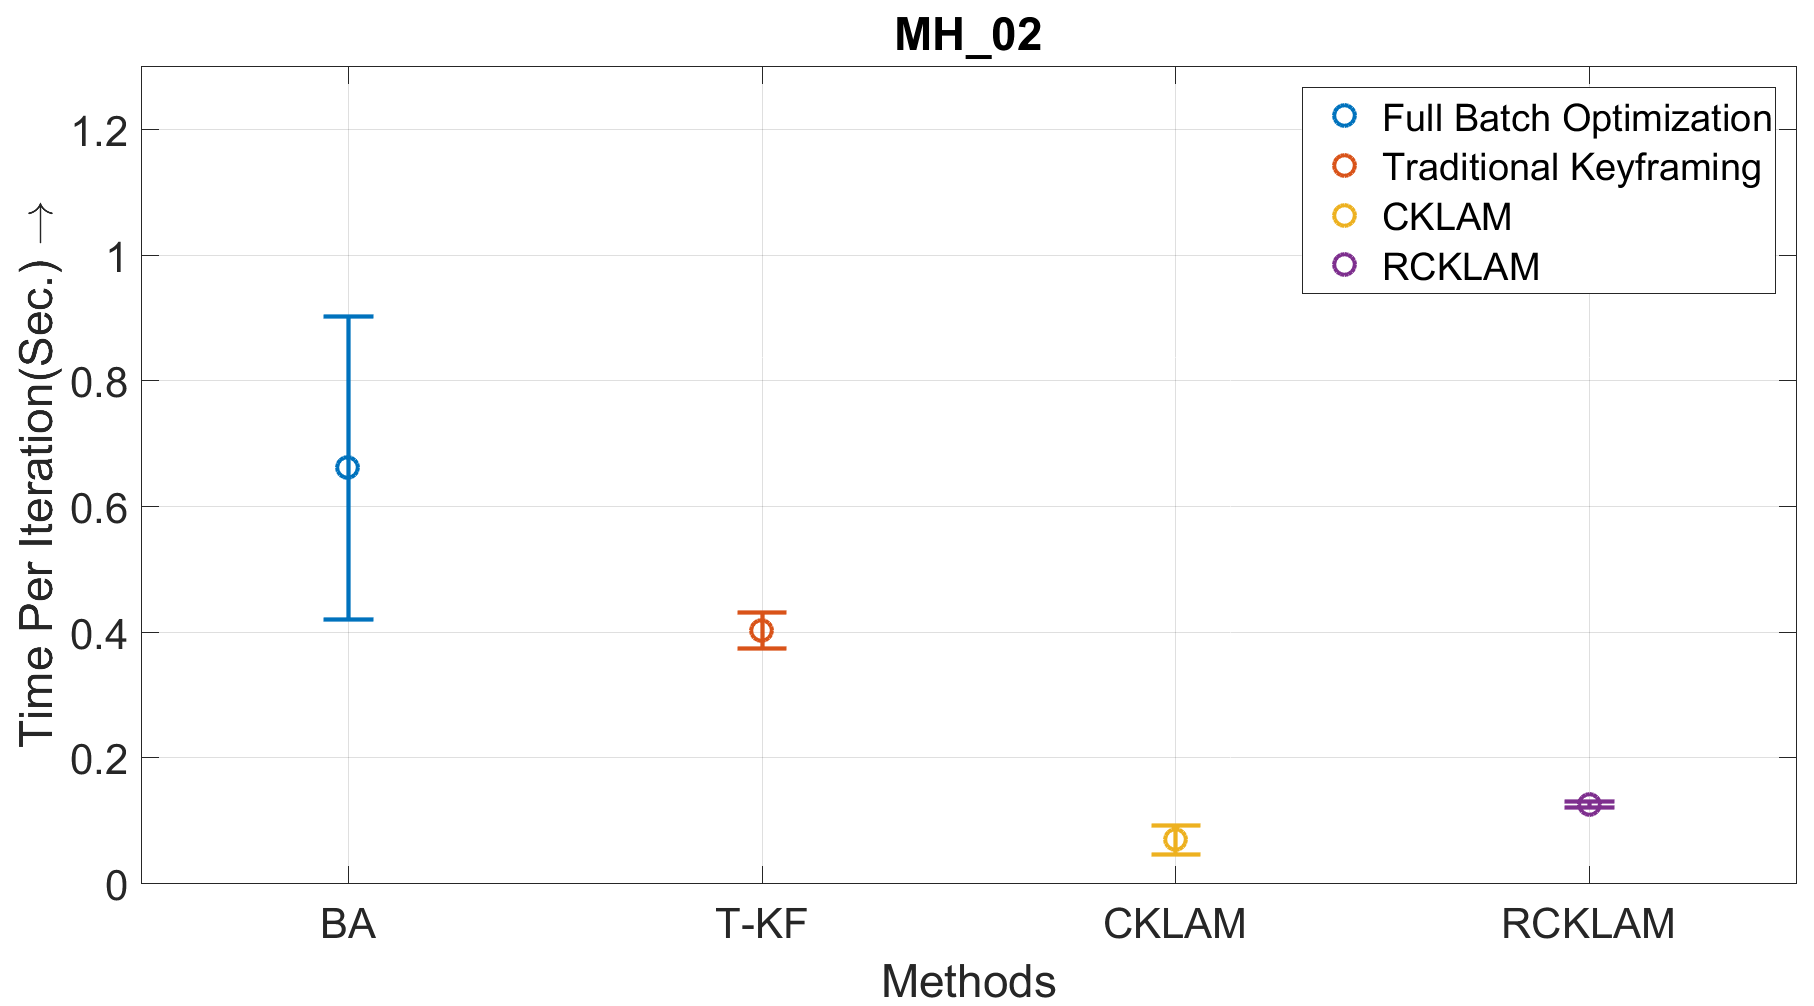
\includegraphics[width=1.00\textwidth]{images/MethodComparisonTimeMH02.png}
	\label{fig:MethodComparisonTimeMH02}
  \caption{Data set MH\_02 from EuRoC \cite{Burri25012016} data set collection. Same experiment as in fugre \ref{fig:MethodComparisonTimeMH01}. In this map $104$ frames were selected as key-frames out of $752$ vertices. The reduction in number of parameters is the main contributor towards the reduction in computational complexity.}
\end{figure}

\begin{figure}
	\centering
		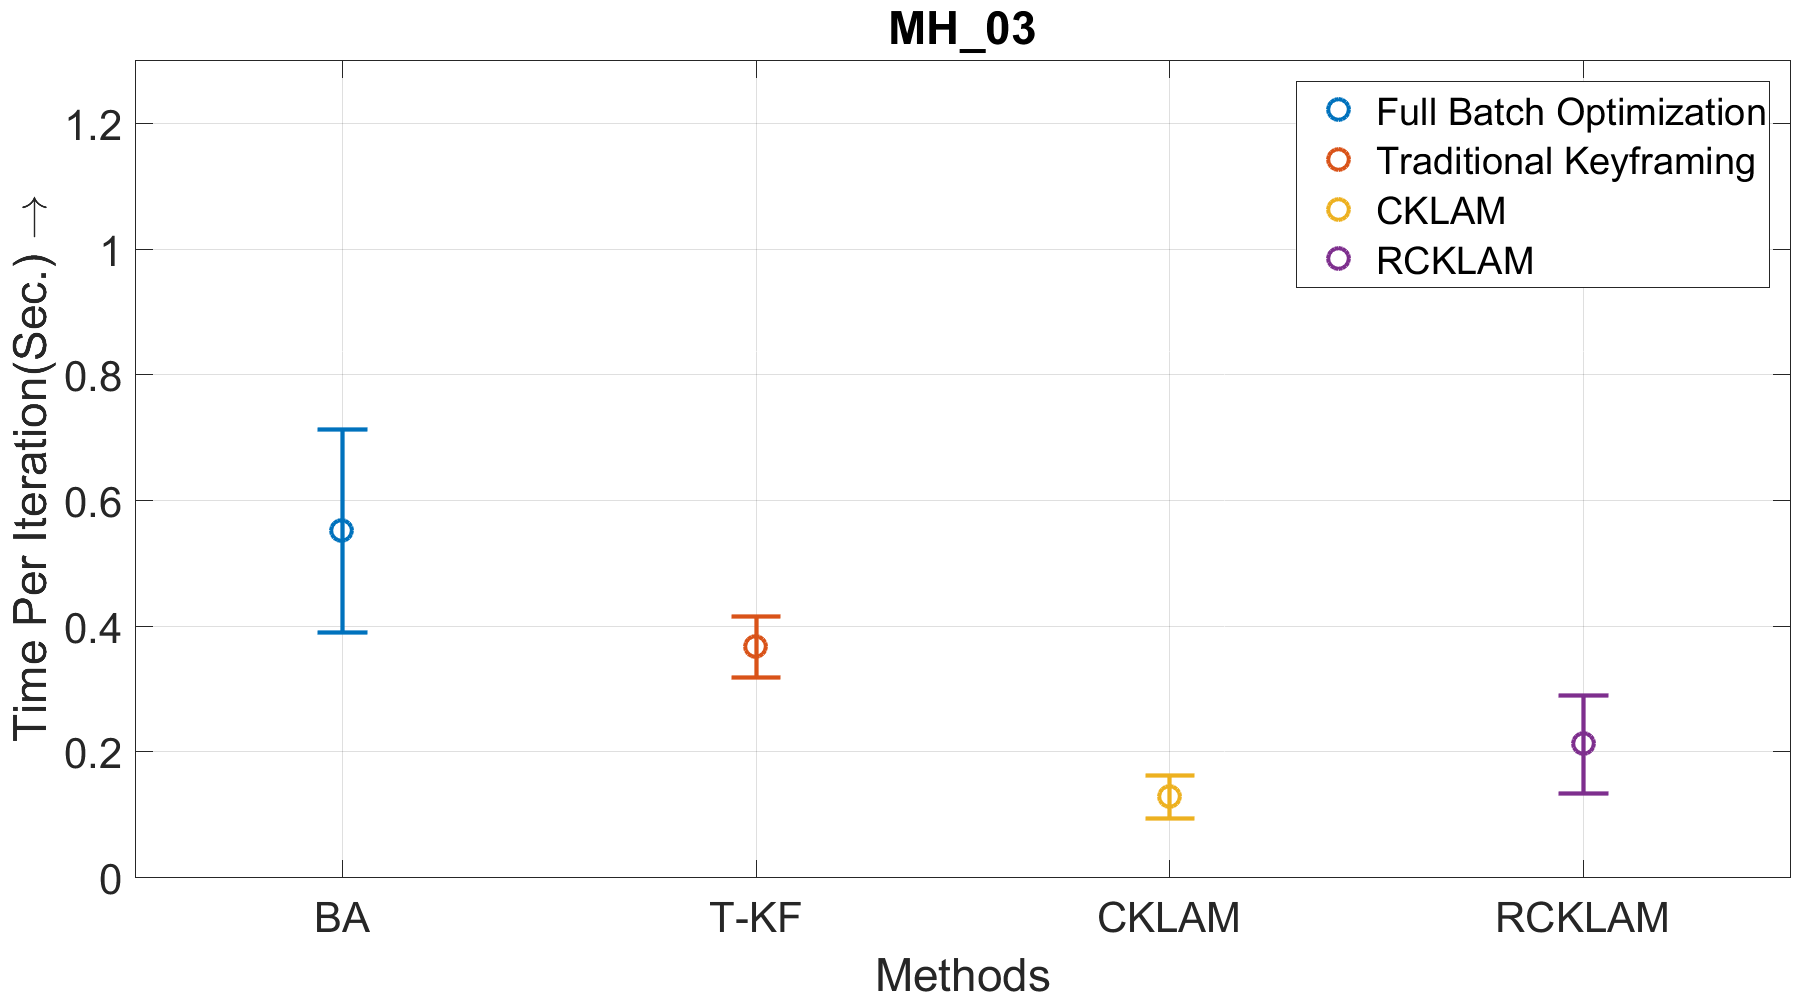
\includegraphics[width=1.00\textwidth]{images/MethodComparisonTimeMH03.png}
	\label{fig:MethodComparisonTimeMH03}
  \caption{Data set MH\_03 from EuRoC \cite{Burri25012016} data set collection. Same experiment as in fugre \ref{fig:MethodComparisonTimeMH01}. In this map $160$ frames were selected as key-frames out of $667$ vertices. The reduction in number of parameters is the main contributor towards the reduction in computational complexity.}
\end{figure}

\chapter{Conclusion}
\label{sec:conclusion}
In this dissertation we present RCKLAM an extension to CKLAM, which is an approximate MAP estimator based algorithm to reduce Bundle Adjustment cost drastically. A realization of the CKALM algorithm was also achieved during this thesis work. In order to reduce complexity both CKLAM and RCKLAM estimates pose of the key-frames and landmarks seen from key-frames. CKLAM instead of discarding information from non-key-frames projects them on to the key frames and achieves improved solution quality. More over CKLAM maintains sparsity of the information matrix that results from the information projection, and hence the batch optimization that follow can be solved efficiently. To verify the correctness of the implementation of the CKLAM method, we have compared its performance against the full batch optimization. The results show that CKLAM not only achieves substantial speed up but also attains an estimation accuracy close to that of the full batch optimization method.

However since CKLAM projects information on to the absolute poses of the key-frames themselves, while information from non-key-frame poses only constrain the relative transformation between key-frames, the problem becomes over constrained after application of CKLAM. This makes the optimization process become overconfident in its estimate and new information such as loop closure information is not propagated through out the map efficiently. RCKLAM addresses this issue by projecting the non-key-frame information onto the relative pose between key-frames. Both with simulated and real life experiments it has been shown that RCKLAM achieves as good estimation accuracy as full batch optimization and has a computational complexity which is very close to that of CKLAM. It also has been shown that in certain loop closure situation RCKLAM performs considerably better than CKLAM.

There lies a few interesting line in which the work can be further extended and achieve even better performance. One such continuation would be to explore if RCKLAM can be performed in an online fashion, i.e. along with the sliding window estimator. In that case the computation cost of RCKLAM information projection would get eliminated and the speed difference margin with batch optimization will be widened. Further more instead of formulating RCKLAM as a two step process it can possibly be formulated as a single step algorithm, in which case we will not only reduce computational complexity resulting from fewer linearization and quadratization process but also get rid of approximation errors.